\section{Reasoning Segmentation and Pixel Grounding}
\label{sec:reasoning-segmentation}

The previous section reviewed promptable and grounded segmentation, where the target is usually specified by a category name, referring expression, visual prompt, region, or grounded dialogue turn. This section studies the third main technical route: reasoning segmentation. Its central objective is to infer the target before producing the mask. In this setting, the input may contain implicit intent, commonsense, spatial relations, multiple possible referents, false premises, task guidelines, or a multi-step instruction. The output is therefore not only a mask, but often a response, a rationale, a rejection decision, or an intermediate grounding trace that must remain faithful to the visual evidence.

Existing work can be broadly grouped into four routes, as summarized in Table~\ref{tab:reasoning-methods}. The first route equips MLLMs with mask outputs through segmentation tokens, codebook tokens, pixel decoders, or mask-aware interfaces. The second route decomposes perception and reasoning, transforming descriptions, candidate regions, or intermediate plans into final masks. The third route optimizes reasoning and segmentation with RL, preference learning, or reward signals. The fourth route controls hallucination and grounded dialogue by testing whether generated language is visually supported and whether invalid queries should be rejected. These routes share a common tension: language reasoning increases flexibility, but pixel grounding decides whether that reasoning is actually useful for segmentation.

\begin{table*}[t]
\centering
\small
\setlength{\tabcolsep}{4pt}
\renewcommand{\arraystretch}{1.32}
\caption{Representative reasoning segmentation and pixel-grounding methods. The table indexes Section~\ref{sec:reasoning-segmentation}; detailed limitations are discussed in the corresponding subsections.}
\label{tab:reasoning-methods}
\begin{tabularx}{\textwidth}{>{\raggedright\arraybackslash}p{0.17\textwidth}>{\raggedright\arraybackslash}X>{\raggedright\arraybackslash}p{0.27\textwidth}>{\raggedright\arraybackslash}p{0.27\textwidth}}
\toprule
Route & Representative methods & Foundation and output setup & Key idea \\
\midrule
Segmentation-token MLLMs & LISA~\citep{xlaiLisaReasoningSegmentation2024}; LLM-Seg~\citep{jwangLlmsegBridgingImage2024}; GSVA~\citep{xiaGsvaGeneralizedSegmentation2024}; READ~\citep{qianReasoningAttendTry2025} & LLaVA-like MLLMs with SAM, Mask2Former, or proposal selectors; \texttt{<SEG>} tokens, proposal selection, multi-mask tokens, or rejection tokens & Introduces reasoning segmentation by linking MLLM hidden states, generated segmentation tokens, or selected proposals to mask outputs. \\
Pixel decoder and codebook interfaces & PixelLM~\citep{renPixellmPixelReasoning2024}; OMG-LLaVA~\citep{zhangOmgllavaBridgingImagelevel2024}; VITRON~\citep{feiVitronUnifiedPixellevel2024}; UniPixel~\citep{liuUnipixelUnifiedObject2026}; ALTo~\citep{wangAltoAdaptivelengthTokenizer2026} & MLLMs with pixel decoders, codebook tokens, universal segmentation encoders, or adaptive mask tokenizers; visual prompts and mask-grounded responses & Expands the mask interface from a single output token to decoder, codebook, or adaptive-token designs for multi-target pixel reasoning. \\
Instruction and complex grounding data & Ground-V~\citep{zongGroundvTeachingVlms2025}; InstructSeg~\citep{weiInstructsegUnifyingInstructed2025}; MMR~\citep{jangMmrLargescaleBenchmark2025}; GroundingSuite~\citep{huGroundingSuiteMeasuringComplex2025} & Teacher models, multi-task visual segmentation, and grounded instruction data; complex instructions, multi-target masks, part references, or image-video outputs & Scales supervision and evaluation for hallucinated references, multi-granularity grounding, and image/video instruction segmentation. \\
Perception-reasoning decomposition & LLM-Seg~\citep{jwangLlmsegBridgingImage2024}; GroundingAgent~\citep{luoConnectingDotsTrainingFree2026}; Pixels-to-Logic~\citep{huangPixelsLogicPerceptionReasoning2026}; R$^2$S~\citep{ningEnhancingSpatialReasoning2025} & Mask proposals, open-vocabulary perception modules, LLM reasoning, point-cloud or scene representations; candidate selection, scene graphs, logic, or relevant-element selection & Separates perception from reasoning so that intermediate candidates, descriptions, or logical structures can be inspected before mask selection. \\
RL and preference optimization & POPEN~\citep{zhuPopenPreferencebasedOptimization2025}; TPO~\citep{yanTaskPreferenceOptimization2025}; LENS~\citep{zhuLensLearningSegment2026}; RISE~\citep{zhouReasoningImplicitSelfsupervised2026}; SAM-R1~\citep{huangSamr1LeveragingSam2026} & LVLM/MLLM backbones with SAM or SAM2; GRPO/DPO-style optimization, preference-ranked responses, CoT formats, box rewards, segment rewards, or SAM feedback & Optimizes reasoning format and mask quality with reward or preference signals beyond ordinary supervised fine-tuning. \\
Dialogue, rejection, and hallucination control & SeeSaySeg~\citep{wuSeeSaySegment2024}; GSVA~\citep{xiaGsvaGeneralizedSegmentation2024}; LLaVA-Grounding~\citep{zhangLlavagroundingGroundedVisual2024}; GLaMM~\citep{rasheedGlammPixelGrounding2024}; VBackChecker~\citep{guoSeeingBelievingRichContext2026}; guideline-consistent segmentation~\citep{vvatsGuidelineConsistentSegmentationMultiAgent2026} & Grounded MLLMs with rejection tokens, backward grounding, or multi-agent refinement; feedback, grounded chat, consistency checking, or guideline critique & Moves reasoning segmentation from always-segment behavior toward verify-then-segment interaction with grounded responses and rejection decisions. \\
\bottomrule
\end{tabularx}
\end{table*}

\subsection{MLLM-guided segmentation}

MLLM-guided segmentation aims to give a language model the ability to produce masks while preserving its instruction-following and reasoning behavior. LISA is the canonical starting point of this route. It defines reasoning segmentation as mask prediction under a complex and implicit query, introduces ReasonSeg for evaluation, and adds a special \texttt{<SEG>} token whose final-layer embedding is decoded into a segmentation mask~\citep{xlaiLisaReasoningSegmentation2024}. This design is important because it makes segmentation a language-generation event: the model first reasons in the MLLM space, then a selected hidden state becomes the bridge to a mask decoder.


Fig.~\ref{fig:reasoning-lisa-placeholder} should be read as the mechanism counterpart to the promptable interfaces in Section~\ref{sec:promptable-grounded-segmentation}. SAM or a segmentation decoder still supplies spatial masks, but the target selection is now mediated by language reasoning. LLM-Seg follows a more modular version of the same idea: it connects an LLM with SAM through mask proposal selection and uses an automatic generation pipeline to build LLM-Seg40K, showing that reasoning segmentation depends as much on scalable instruction-mask data as on architecture~\citep{jwangLlmsegBridgingImage2024}. GSVA extends the token interface to generalized referring expression segmentation by allowing multiple mask references and by learning a rejection token for absent targets~\citep{xiaGsvaGeneralizedSegmentation2024}. READ then analyzes how the \texttt{<SEG>} token attends to image tokens and uses similarity-derived points as plug-in guidance, suggesting that segmentation tokens do not merely mark output format; they can carry object-level semantic attention~\citep{qianReasoningAttendTry2025}.



The next step is to improve mask capacity beyond a single hidden token. PixelLM replaces the heavy external segmentation dependence with a lightweight pixel decoder and segmentation codebook. The codebook stores learnable tokens for different visual scales, and the decoder turns their hidden embeddings into masks; this supports multi-target reasoning and reduces reliance on separate segmentation models~\citep{renPixellmPixelReasoning2024}. OMG-LLaVA uses a universal segmentation method as the visual encoder and injects image information, perception priors, and visual prompts into an LLM so that image-level, object-level, and pixel-level reasoning can be handled in one framework~\citep{zhangOmgllavaBridgingImagelevel2024}. VITRON generalizes further by combining image, video, and pixel-level regional modules with backend visual specialists for understanding, generation, segmentation, and editing~\citep{feiVitronUnifiedPixellevel2024}. UniPixel and ALTo continue this trend by making masks and visual pointers part of the MLLM interaction: UniPixel conditions later reasoning on intermediate pixel-level pointers, while ALTo uses adaptive-length mask tokenization to trade mask quality against token cost~\citep{liuUnipixelUnifiedObject2026,wangAltoAdaptivelengthTokenizer2026}.

In summary, MLLM-guided segmentation is effective because it turns a mask into an output that can be requested, discussed, rejected, or revised in language. Its limitation is that the mask interface can become a bottleneck. A single \texttt{<SEG>} token may not capture multiple regions or fine boundaries; a proposal selector cannot recover missing candidates; a codebook or decoder can improve capacity but introduces new training, token-budget, and efficiency choices. Thus, when comparing MLLM-guided methods, one should report not only the language backbone but also the mask interface, number of segmentation tokens, decoder type, external segmenter, and whether reasoning data or only reasoning-free data is used.


\begin{figure*}[htbp]
    \centering
    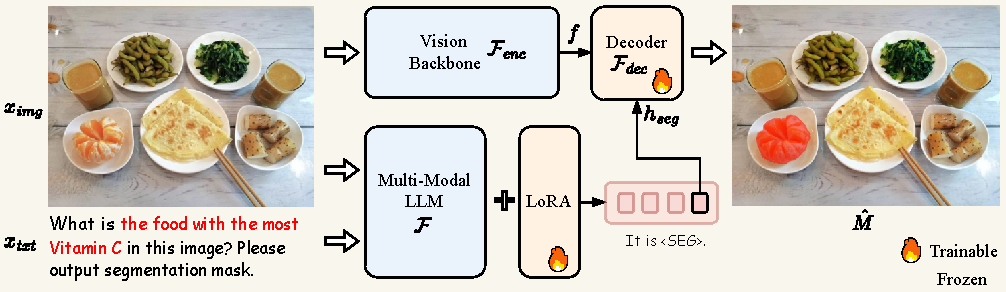
\includegraphics[width=0.98\textwidth]{Fig/fig_LISA.pdf}
    \caption{LISA's embedding-as-mask pipeline for reasoning segmentation. This placeholder should be replaced by the original pipeline figure from LISA, which shows the image and text query entering an MLLM, the generated \texttt{<SEG>} token, and the decoding of its hidden embedding into a segmentation mask~\citep{xlaiLisaReasoningSegmentation2024}.}
    \label{fig:reasoning-lisa-placeholder}
\end{figure*}


\subsection{Reasoning-to-mask generation}

Reasoning-to-mask generation studies how an inferred target is transformed into a spatial output. The key difference from ordinary referring segmentation is that the query may not name the target directly. It may ask for the object that satisfies a relation, a function, a scene constraint, a commonsense clue, or a domain rule. This makes the intermediate representation important: the system must decide whether to reason over text, boxes, masks, region proposals, scene descriptions, or latent hidden states.

One route is proposal selection. LLM-Seg uses SAM proposals and lets the language reasoning module select the target mask, which makes the process interpretable but dependent on proposal recall~\citep{jwangLlmsegBridgingImage2024}. GroundingAgent extends this philosophy into a training-free agentic grounding framework. It combines open-vocabulary detectors, MLLMs, and LLMs in an iterative process that refines candidate regions through semantic and spatial analyses~\citep{luoConnectingDotsTrainingFree2026}. From Pixels to Logic converts visual perception into a rich textual scene representation and then applies a reasoning language model for open-world referring expression comprehension, including multiple, absent, or novel referents~\citep{huangPixelsLogicPerceptionReasoning2026}. These methods trade end-to-end compactness for transparency: the reader can inspect candidate regions and reasoning decisions, but failures in detection, captioning, or scene abstraction may still dominate the final result.

Another route is instruction or data scaling. Ground-V constructs instruction-response pairs linked to pixel annotations and explicitly targets hallucinated references, multi-object cases, reasoning, multi-granularity, and part-level references~\citep{zongGroundvTeachingVlms2025}. InstructSeg defines instructed visual segmentation as the union of referring and reasoning segmentation across images and videos, using object-aware video perception and multi-granularity text fusion for a single end-to-end pipeline~\citep{weiInstructsegUnifyingInstructed2025}. MMR moves the benchmark side toward multi-target and multi-granularity reasoning segmentation, where a model must output masks at different levels of object and part granularity rather than only one referred object~\citep{jangMmrLargescaleBenchmark2025}. GroundingSuite plays a similar role for pixel grounding by measuring complex multi-granular grounding under diverse expressions~\citep{huGroundingSuiteMeasuringComplex2025}.

A third route makes reasoning explicitly structured. R$^2$S decomposes complex 3D spatial reasoning into relevant-element identification followed by instruction processing with visual priors, showing that reasoning segmentation is not limited to 2D images~\citep{ningEnhancingSpatialReasoning2025}. Guideline-consistent segmentation uses a Worker-Supervisor multi-agent loop: the worker generates a segmentation, the supervisor critiques it against retrieved guidelines, and a lightweight stop policy decides whether refinement should continue~\citep{vvatsGuidelineConsistentSegmentationMultiAgent2026}. This pattern is valuable for real annotation or domain settings, where the correct mask is defined not only by an object name but also by paragraph-length rules.

Reasoning-to-mask generation therefore exposes a design choice. End-to-end token or decoder models are compact and can be optimized jointly, but their reasoning traces are hard to audit. Decomposition methods are more inspectable, but their quality depends on the perceptual modules and intermediate abstractions. Data-scaling methods can improve coverage, but automatically generated reasoning data may import teacher-model biases. The most convincing future systems will likely combine these advantages: explicit enough to verify, dense enough to produce accurate masks, and scalable enough to cover implicit and multi-target instructions.

\begin{figure*}[htbp]
    \centering
    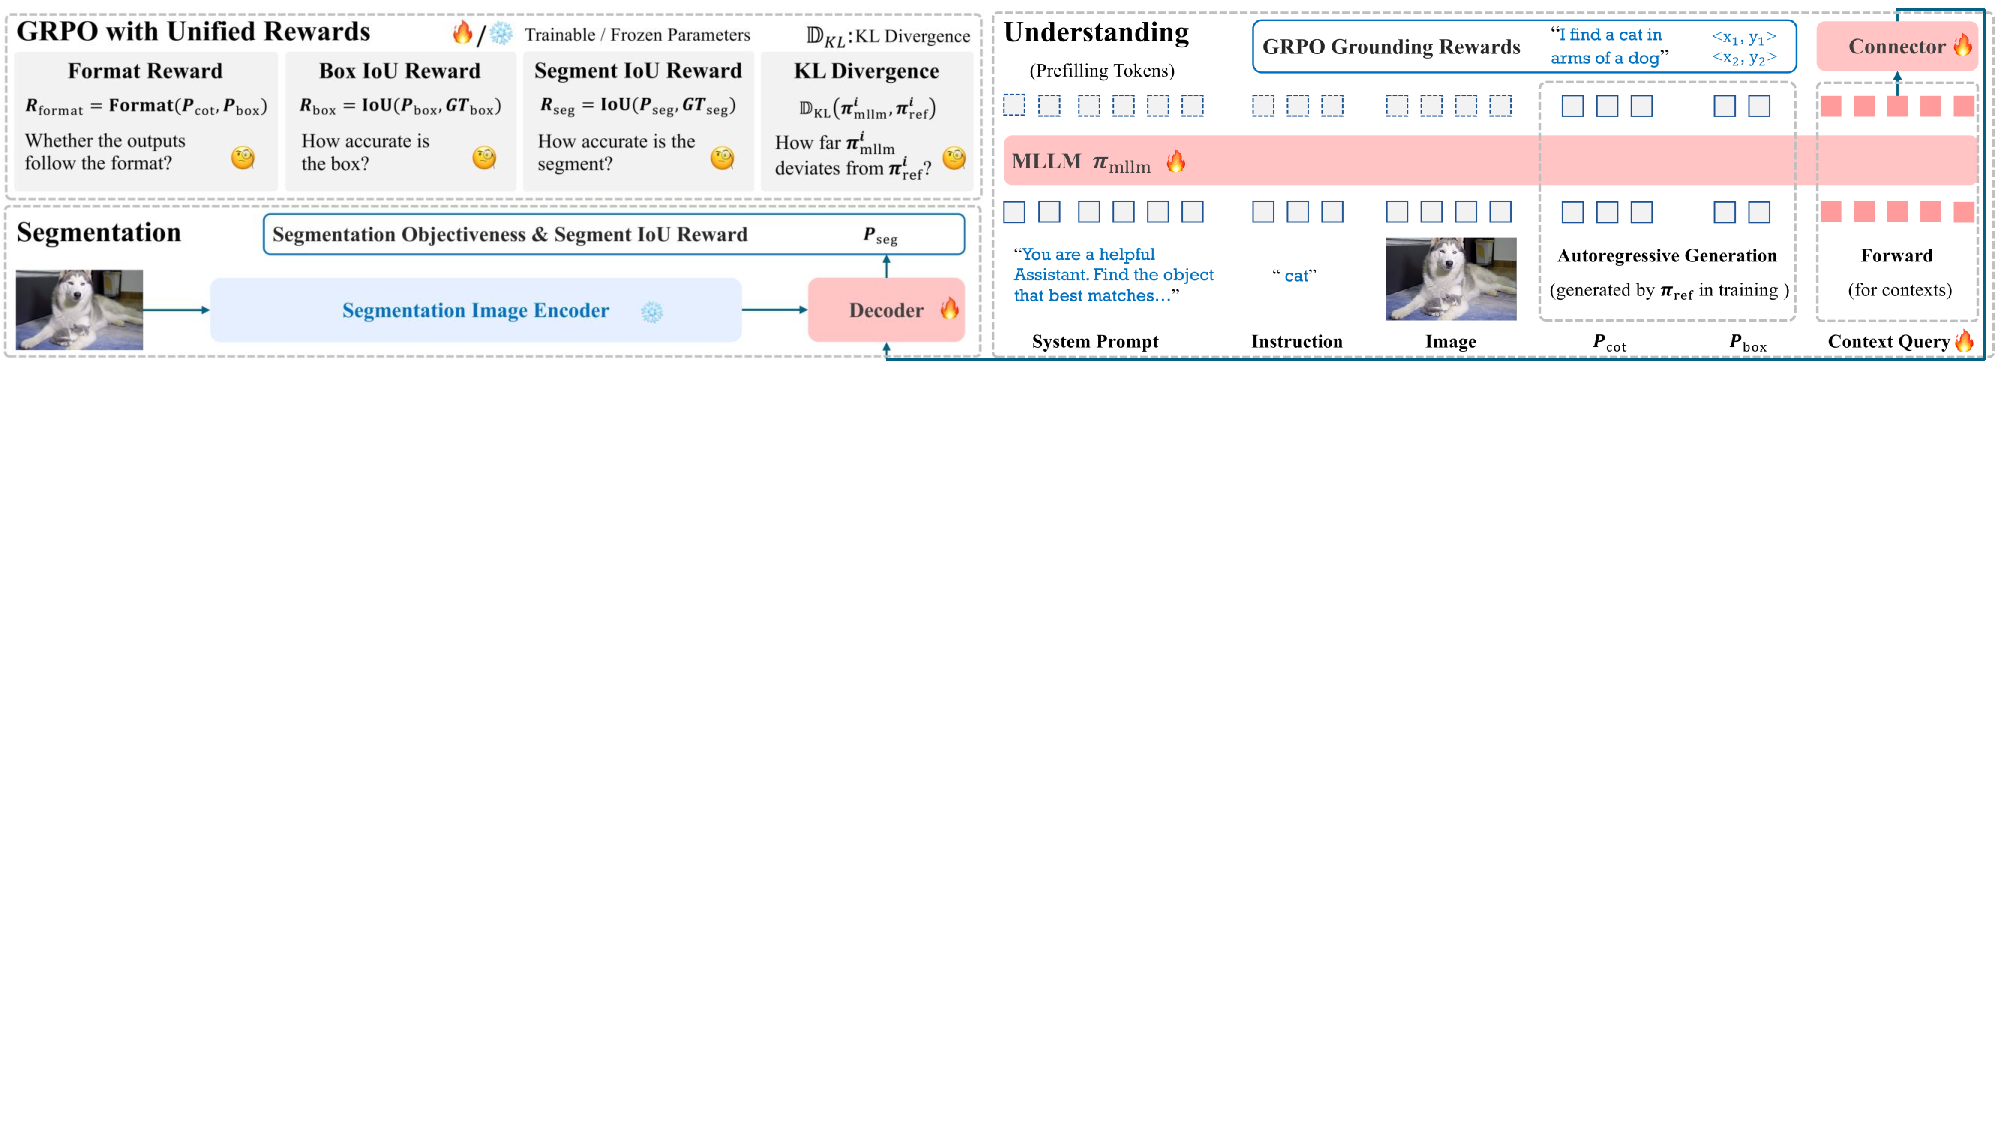
\includegraphics[width=0.98\textwidth]{Fig/fig_LENS.pdf}
    \caption{LENS RL framework for text-prompted segmentation. This placeholder should be replaced by the original LENS overview figure, which contrasts supervised \texttt{<seg>} prompting with an end-to-end RL framework using context queries, a connector to SAM, and unified rewards over reasoning format, localization, and mask quality~\citep{zhuLensLearningSegment2026}.}
    \label{fig:reasoning-lens-placeholder}
\end{figure*}

\subsection{RL and preference optimization}

Supervised fine-tuning teaches a model to imitate instruction-mask pairs, but reasoning segmentation often requires choosing among multiple plausible rationales and masks. RL and preference optimization address this gap by defining what counts as a better response, a better target, or a better mask. This route became especially important after early MLLM-based methods exposed two coupled failure modes: text responses can hallucinate, and masks can be imprecise even when the language response appears correct.



POPEN is a representative preference-based method. Built on an LVLM-based reasoning segmentation framework, it collects preference data for both text semantics and segmentation embeddings, then uses preference optimization and a preference-based ensemble to reduce hallucination and improve mask accuracy~\citep{zhuPopenPreferencebasedOptimization2025}. The important writing point is not only that POPEN optimizes preferences, but that it separates two preference sources: language-side corrections and mask-side ranking. This makes it better aligned with the dual-output nature of reasoning segmentation.



LENS provides a clearer RL formulation, as indicated by the planned Fig.~\ref{fig:reasoning-lens-placeholder}. It couples an MLLM with SAM through context queries and a connector, then applies GRPO-style optimization with rewards spanning output format, box localization, and segment IoU~\citep{zhuLensLearningSegment2026}. Compared with a single \texttt{<SEG>} token, this design uses the chain-of-thought trace and grounding box as richer priors for mask generation. RISE pushes the supervision question further by showing that instruction segmentation can emerge from a simple semantic-alignment reward without ground-truth masks, using GRPO to unlock implicit compositional reasoning~\citep{zhouReasoningImplicitSelfsupervised2026}. SAM-R1 instead uses SAM as a reward provider for fine-grained segmentation-oriented reasoning, demonstrating that a foundation segmenter can supervise reasoning optimization without being only an inference-time mask generator~\citep{huangSamr1LeveragingSam2026}.

Preference and reward learning also appear beyond strict 2D image segmentation. Task Preference Optimization introduces learnable task tokens and differentiable task preferences derived from fine-grained vision tasks, improving MLLM alignment with visual outputs across task heads~\citep{yanTaskPreferenceOptimization2025}. Fine-grained preference optimization studies spatial reasoning in VLMs more generally and is relevant because many segmentation errors are actually spatial-reasoning errors before they are boundary errors~\citep{shenFinegrainedPreferenceOptimization2026}. In extended scenarios, MedReasoner, Affordance-R1, VideoSeg-R1, and Omni-R1 apply similar RL logic to clinical grounding, affordance reasoning, video object segmentation, and omnimodal reasoning, which will be discussed in Section~\ref{sec:extended-scenarios}.

The advantage of RL and preference optimization is that they can align the model with outcomes that supervised labels do not fully describe: response format, rationale usefulness, target localization, mask quality, rejection behavior, and efficiency. The limitation is reward faithfulness. A high mask-IoU reward may not prove that the chain of thought caused the mask; a format reward may produce well-structured but shallow rationales; a preference dataset may encode annotator or teacher-model bias. Therefore, RL-based reasoning segmentation should be evaluated with both mask metrics and faithfulness checks, not only with cIoU or gIoU.

\subsection{Grounded dialogue and hallucination control}

Grounded dialogue changes the default assumption from ``always return a mask'' to ``answer, ground, segment, or reject as appropriate.'' This is necessary because reasoning segmentation queries can be invalid or misleading. A user may ask for an object that is absent, use a wrong attribute, refer to multiple targets, or request a region that violates labeling guidelines. In such cases, returning a confident mask is a failure even if the mask looks visually plausible.

SeeSaySeg directly targets false premises. It teaches LMMs to first see whether the object exists, then say useful corrective feedback when it does not, and finally segment only when a valid target is present~\citep{wuSeeSaySegment2024}. GSVA introduces an explicit rejection token for generalized segmentation, allowing the model to handle multiple or absent referents rather than forcing every expression into a single mask~\citep{xiaGsvaGeneralizedSegmentation2024}. These works are important because they broaden the evaluation target: a reasoning segmentation model should be rewarded for refusing a false query just as much as for segmenting a valid one.

Grounded visual chat methods expose a second failure mode: generated text and masks can disagree. LLaVA-Grounding connects generated visual-chat responses with spatial grounding, while GLaMM interleaves natural-language responses with object segmentation masks~\citep{zhangLlavagroundingGroundedVisual2024,rasheedGlammPixelGrounding2024}. These interfaces are more flexible than single-mask predictors, but they require mask-response consistency. A response can mention the correct object but attach a wrong mask; it can describe an unseen object; or it can ground only salient nouns while ignoring relations and attributes. GroundingSuite and Ground-V both respond to this problem by scaling multi-granular pixel grounding data and evaluation~\citep{huGroundingSuiteMeasuringComplex2025,zongGroundvTeachingVlms2025}.

Hallucination checking makes this consistency problem explicit. VBackChecker verifies MLLM responses through backward visual grounding: generated rich-context descriptions are checked against pixel-level grounding masks and hard negative samples~\citep{guoSeeingBelievingRichContext2026}. Guideline-consistent segmentation addresses a related but more rule-driven case. Instead of checking whether a caption is grounded, it checks whether a mask follows long textual labeling guidelines through iterative worker-supervisor refinement~\citep{vvatsGuidelineConsistentSegmentationMultiAgent2026}. Together, these methods show that reasoning segmentation is becoming a verification problem as much as a prediction problem.

Grounded dialogue and hallucination control therefore form the reliability layer of reasoning segmentation. They ask whether the system knows when not to segment, whether it can explain uncertainty, whether the output mask supports the generated response, and whether the response obeys domain or dataset rules. This route connects directly to Section~\ref{sec:comparison-discussion}, where reasoning capability must be separated from grounding faithfulness.

\subsection{Summary and discussion}

Several conclusions can be drawn from this section. First, reasoning segmentation is not simply referring expression segmentation with longer text. Its defining step is target inference: the model must decide what should be segmented from implicit intent, relations, commonsense, guidelines, or dialogue context before mask generation begins.

Second, the field is moving from single-token mask triggering toward richer mask interfaces. LISA's \texttt{<SEG>} token established the embedding-as-mask paradigm, but later systems add proposal selection, rejection tokens, codebook tokens, pixel decoders, adaptive mask tokenizers, context queries, and grounded responses. These designs increase capacity, but they also create new reporting requirements: token budget, decoder type, prompt source, external segmenter, and target-data usage should be made explicit.

Third, RL and preference optimization are becoming central because reasoning segmentation is a dual-output alignment problem. The language response, reasoning trace, target localization, and mask all have to be right. Reward and preference methods are promising, but they must be audited for faithfulness; otherwise, a model may learn to produce convincing rationales that merely accompany rather than cause correct masks.

Finally, reasoning segmentation brings reliability concerns to the surface. False premises, absent targets, multi-target references, hallucinated objects, and guideline conflicts cannot be evaluated by mask IoU alone. A mature benchmark should therefore combine segmentation accuracy, rejection accuracy, response correctness, mask-response consistency, and efficiency. The next section extends these questions to video, 3D, remote-sensing, medical, affordance, and embodied scenarios, where temporal, spatial, and domain-specific constraints further stress-test the same reasoning-to-mask pipeline.
